\chapter{Implementation}

\textbf{Phase 1 Scope and Objectives:} This chapter presents the initial implementation phase of the MRAG system. In Phase 1, the primary focus is on \textbf{establishing and validating the core system architecture}, including the data processing pipeline, embedding strategies, and retrieval mechanisms. The implementation prioritizes architectural feasibility and functional correctness. Advanced considerations such as production-grade application development, optimized database storage solutions, and comprehensive system optimization are deliberately deferred to Phase 2. This phased approach allows for iterative refinement based on empirical evaluation of the foundational architecture before committing to infrastructure-level optimizations.

This chapter details the practical implementation of the core system architecture. We describe the system design, data processing pipeline, and key implementation components that enable efficient document processing and retrieval.

\section{Architecture Design}

The Unified MRAG Pipeline is architected as a modular, resource-optimized system designed to handle the complete lifecycle of document intelligence from raw ingestion to semantic generation. The system deviates from traditional monolithic designs by adopting a \textbf{Layered Service Architecture}, decoupling the retrieval logic from the generation logic, and utilizing a file-system-based state management approach for portability.

The architecture is composed of four primary layers:

\textbf{1. Interface Layer (API Gateway)}

The entry point to the system is a high-performance RESTful API built on \textbf{FastAPI}. This layer is responsible for request validation, concurrency management, and protocol serialization.
\begin{itemize}
    \item \textbf{Asynchronous I/O}: To prevent thread blocking during heavy file uploads, the \texttt{/api/upload} and \texttt{/api/process} endpoints utilize Python's \texttt{async/await} pattern combined with FastAPI's \texttt{BackgroundTasks}. This allows the server to immediately acknowledge receipt of a request while heavy computation (ETL) occurs in a separate thread pool.
    \item \textbf{State Management}: To minimize latency during search operations, the system utilizes a \textit{Lifespan Event Handler}. Upon application startup, heavy models (embedding models, cross-encoders, and ColQwen weights) are pre-loaded into GPU memory and stored in the application state (\texttt{app.state}), eliminating initialization overhead per request.
\end{itemize}

\textbf{2. Orchestration Layer}

At the core of the system lies the \texttt{UnifiedRAGPipeline} class. This component acts as the central controller, implementing the \textbf{Facade Pattern} to abstract the complexities of the underlying subsystems.
\begin{itemize}
    \item \textbf{Pipeline Configuration}: The behavior of the orchestrator is dictated by a dynamic YAML configuration (e.g., \texttt{config/default.yaml}). This allows the system to switch between ``Text-Only,'' ``Image-Only,'' or ``Multimodal'' modes without code changes.
    \item \textbf{Dependency Injection}: The orchestrator initializes and injects dependencies into the sub-modules, ensuring that the \textit{RetrieverManager} and \textit{Generator} share the same configuration context (e.g., chunk sizes and overlaps).
\end{itemize}

\textbf{3. Data Processing and Persistence Layer}

Unlike cloud-native solutions that rely on external vector databases (e.g., Pinecone, Milvus), this architecture implements a self-contained \textbf{File-System Artifact Store}. This design choice maximizes data privacy and portability. The storage architecture is organized into a rigid directory hierarchy:

% \begin{verbatim}
% output/
% ├── processing/         # Intermediate ETL artifacts
% │   ├── stage1_normalized/
% │   ├── stage2_media/
% │   ├── stage3_docling/
% │   └── stage4_rag_ready/
% ├── retrieval/          # Text Search Indices
% │   ├── bm25/           # Sparse Inverted Index (.pkl)
% │   ├── dense/          # FAISS Vector Index (.bin)
% │   └── documents.json  # Metadata Catalog
% └── image_retrieval/    # Visual Search Indices
%     └── colqwen/        # Visual Tensor Store
% \end{verbatim}

\textbf{4. Logical Subsystems}

The system logic is divided into two specialized engines that operate in parallel during query execution:

\textbf{Text Retrieval Engine}

This subsystem implements a ``Retrieve-then-Rerank'' pipeline:
\begin{enumerate}
    \item \textbf{Sparse Retrieval}: Uses BM25Okapi to capture keyword-specific relevance.
    \item \textbf{Dense Retrieval}: Uses \texttt{all-MiniLM-L6-v2} to generate 384-dimensional embeddings for semantic search via FAISS (IndexFlatIP).
    \item \textbf{Hybrid Fusion}: A weighted algorithm combines scores ($Score = \alpha \cdot Dense + (1-\alpha) \cdot BM25$).
    \item \textbf{Reranking}: A Cross-Encoder (\texttt{bge-large}) re-evaluates the top $K$ candidates to ensure high precision.
\end{enumerate}

\textbf{Visual Retrieval Engine (ColQwen)}

This subsystem handles non-textual data. Instead of extracting text from images (OCR), it utilizes a Vision-Language Model (ColQwen2).
\begin{enumerate}
    \item \textbf{Rasterization}: PDFs are converted to high-resolution images (150 DPI).
    \item \textbf{Visual Embedding}: The model generates a tensor representation of the visual layout.
    \item \textbf{Just-in-Time Rendering}: During generation, the specific retrieved page is rendered on-the-fly and passed to the Multimodal LLM, allowing the AI to ``see'' charts and diagrams directly.
\end{enumerate}

% \section{Data Normalization}
% Data normalization ensures that heterogeneous input formats are standardized before processing. The system implements a file-system-based normalization strategy located in the \texttt{input} directory.

% Upon upload via the \texttt{/api/upload} endpoint, the following normalization steps are enforced:
% \begin{itemize}
%     \item \textbf{Filename Sanitization}: Incoming files are checked for naming collisions. If a file with the same name exists, the system automatically appends a numerical suffix (e.g., \texttt{file\_1.pdf}) to maintain uniqueness without overwriting existing data.
%     \item \textbf{Format Validation}: The system currently supports PDF and image-based inputs, filtering unsupported MIME types at the entry gate.
%     \item \textbf{Metadata Extraction}: Basic file attributes (size, modification time, MIME type) are extracted and normalized into a standard JSON structure for frontend display.
% \end{itemize}

\section{Data Normalization}

Data normalization is a critical preprocessing step designed to reduce the entropy of input data formats. As illustrated in Figure \ref{fig:normalization}, the system accepts a wide variety of unstructured and semi-structured inputs ranging from multimedia files to office documents and funnels them into a standardized ``RAG-ready'' format.
The normalization pipeline is governed by the \texttt{Processor} module and utilizes a suite of open-source libraries to perform format unification.

Upon upload via the API, raw files undergo immediate sanitization:
\begin{itemize}
    \item \textbf{Filename Sanitization}: To prevent filesystem collisions and encoding errors, filenames are normalized to ASCII characters, and duplicate uploads are handled via an incremental suffix strategy.
    \item \textbf{Type Validation}: The system acts as a gatekeeper, filtering files based on magic numbers to ensure only supported formats proceed to the processing stage.
\end{itemize}


To facilitate both Visual (ColQwen) and Textual (Dense/Sparse) retrieval, all inputs are converted into two canonical formats: \textbf{PDF} (for visual representation) and \textbf{Markdown} (for semantic text content).

The specific normalization strategies per file type are as follows:

% \textbf{Office and Document Formats}

% Legacy office formats (DOC, DOCX, PPT, PPTX, XLS) are often difficult to parse directly. 
% The system utilizes \textbf{LibreOffice} in headless mode (server-side).
% These documents are converted into standard PDF format. This ensures that layout, fonts, and slide structures are preserved visually for the image retrieval engine.


% \textbf{Multimedia (Audio and Video)}

% Video (MP4, AVI) and Audio (WAV, MP3) files contain rich semantic information that must be serialized into text.
% \textbf{MoviePy} is employed to separate audio tracks from video containers.
% The \textbf{OpenAI Whisper} model (Automatic Speech Recognition) processes the audio stream to generate high-fidelity transcripts. These transcripts are saved as Markdown text files, time-stamped to allow for future temporal retrieval.

% \textbf{Structural Parsing (Docling)}

% For complex documents like scientific PDFs, HTML pages, or Table-heavy reports, simple text extraction is insufficient.
% The pipeline integrates \textbf{Docling}, a specialized document parsing library.
% Docling analyzes the document structure to distinguish between headers, paragraphs, and tables.
% It outputs structured \textbf{Markdown} that preserves table boundaries (CSV-style) and document hierarchy. This allows the text chunker to respect semantic boundaries rather than cutting sentences mid-table.


\textbf{Multimedia Processing}

To handle temporal media, the system implements a two-step transformation:
\begin{itemize}
    \item \textbf{Video Extraction}: Raw video files (e.g., MP4) are processed using \textbf{MoviePy}. This extractor separates the visual stream from the audio stream, outputting a \texttt{.WAV} file for transcription and an optional image thumbnail.
    
    \begin{figure}[H]
        \centering
        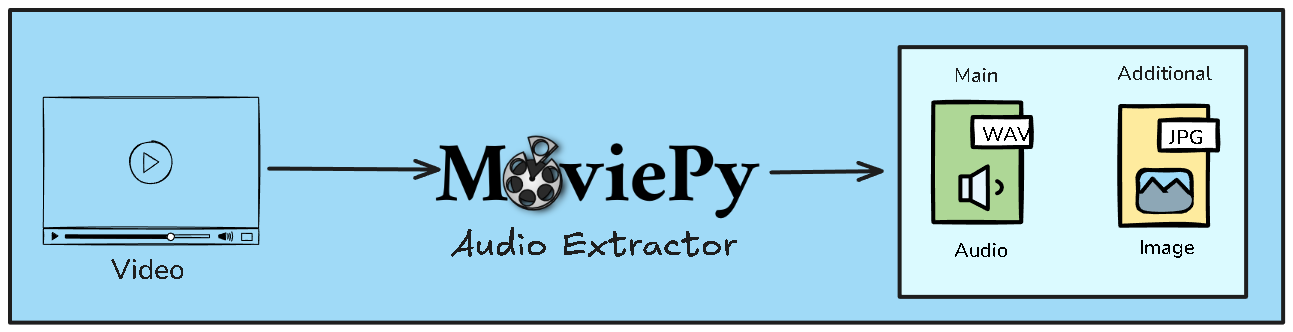
\includegraphics[width=1\textwidth]{img/pdz/23-movipy.png}
        \caption[MoviePy Extraction Process]{MoviePy Extraction Process.}
        \label{fig:movipy_process}
    \end{figure}
    
    \item \textbf{Audio Transcription}: The extracted audio or raw \texttt{.WAV} files are passed to \textbf{OpenAI Whisper} ASR engine. Whisper transcribes the speech to text, which is immediately serialized into \textbf{Markdown} format to preserve semantic structure.
    
    \begin{figure}[H]
        \centering
        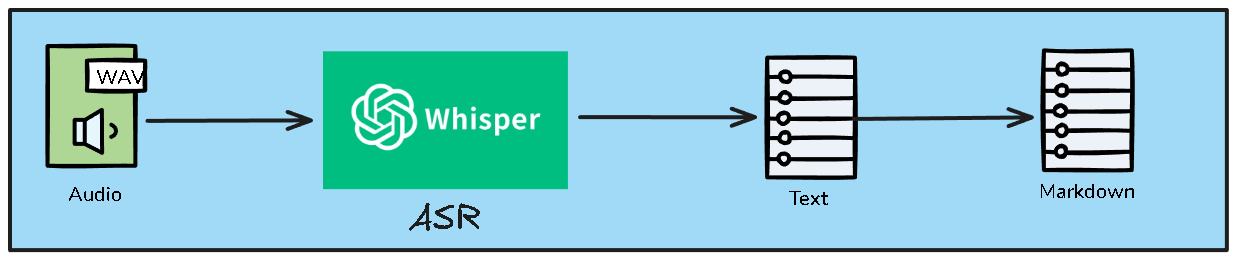
\includegraphics[width=1\textwidth]{img/pdz/24-whisper.png}
        \caption[OpenAI Whisper Audio Transcription Process]{OpenAI Whisper Audio Transcription Process.}
        \label{fig:whisper_process}
    \end{figure}

\end{itemize}

\textbf{Office Document Normalization}

Legacy office formats require conversion before structural analysis. The system utilizes \textbf{LibreOffice} in a headless server environment.
\begin{figure}[H]
    \centering
    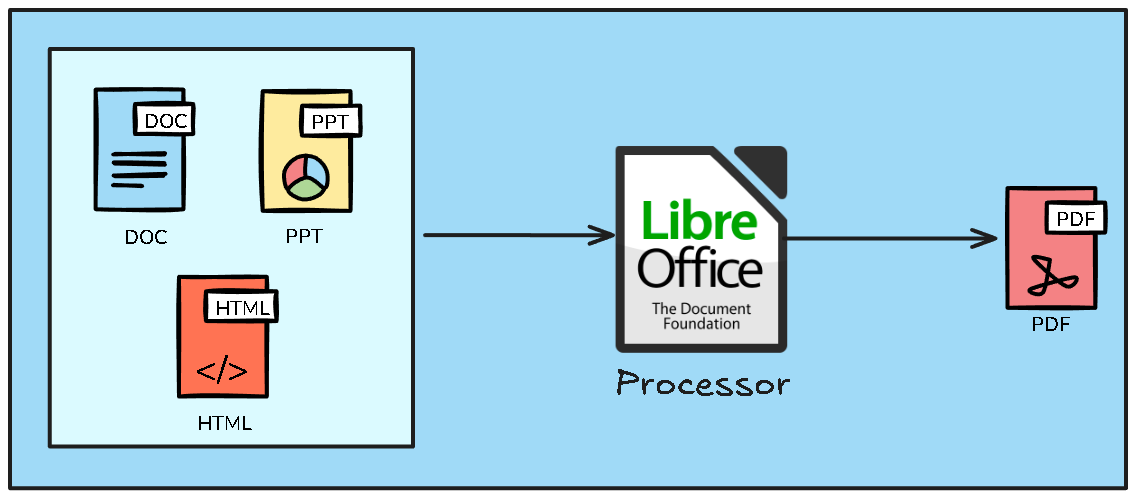
\includegraphics[width=0.7\textwidth]{img/pdz/25-libre.png}
    \caption[LibreOffice Document Conversion Process]{LibreOffice Document Conversion Process.}
    \label{fig:libre_process}
\end{figure}

Formats such as Microsoft Word (.DOC), PowerPoint (.PPT), and HTML are normalized into standard \textbf{PDF} documents to freeze layout and fonts.

\textbf{Complex Document Parsing}

For data-dense documents, the pipeline integrates \textbf{Docling} as the central parsing engine:

\begin{figure}[H]
    \centering
    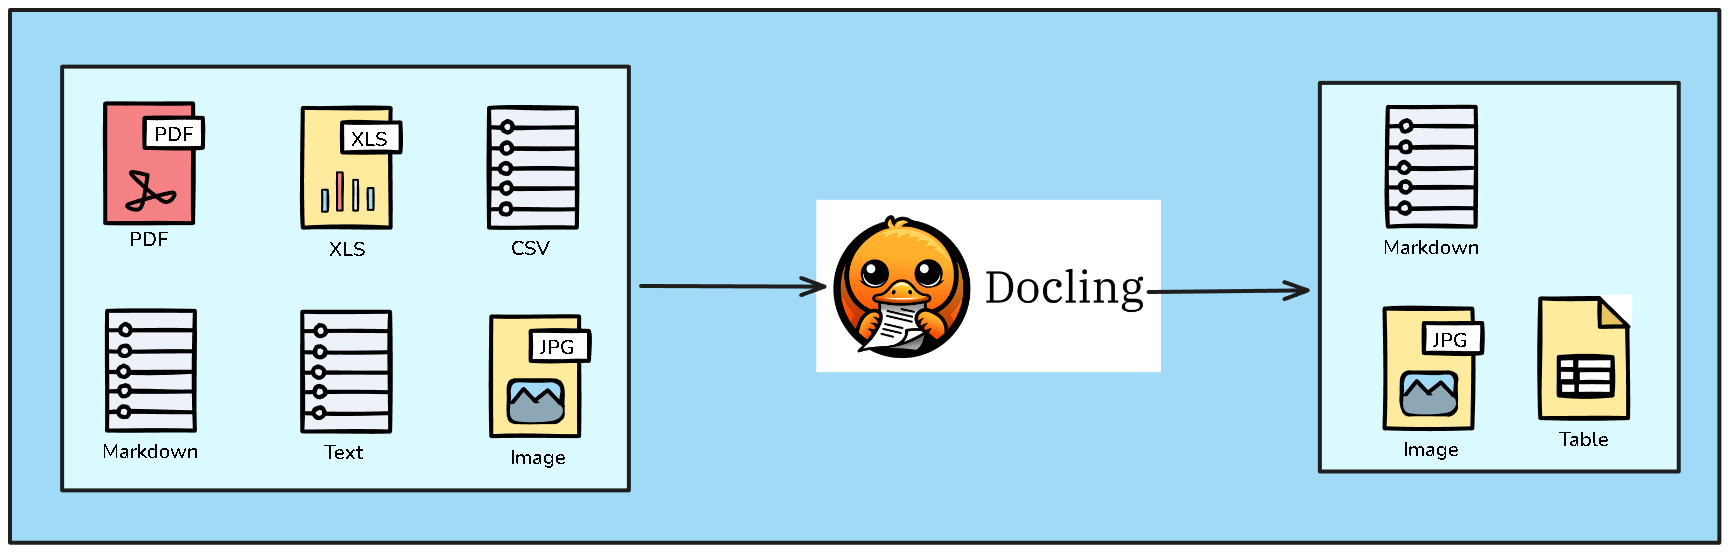
\includegraphics[width=1\textwidth]{img/pdz/26-docling.png}
    \caption[Docling Document Parsing Process]{Docling Document Parsing Process.}
    \label{fig:docling_process}
\end{figure}

\begin{itemize}
    \item \textbf{Inputs}: Handles PDF, Excel (.XLS), CSV, Markdown, Text, and Images.
    \item \textbf{Outputs}: Docling deconstructs these inputs into three distinct normalized artifacts:
    \begin{enumerate}
        \item \textbf{Structured Markdown}: For semantic text analysis.
        \item \textbf{Table Objects}: For preserving row/column relationships.
        \item \textbf{Isolated Images}: For downstream visual indexing.
    \end{enumerate}
\end{itemize}

% \textbf{Output Artifacts}

% Every input file results in a unified set of artifacts in the rag ready directory:
% \begin{enumerate}
%     \item \textbf{PDF}: Used for visual embedding (ColQwen) and user preview.
%     \item \textbf{Structured Markdown}: Used for text embedding (BM25/Dense) and LLM context injection.
%     \item \textbf{Extracted Metadata}: JSON sidecars containing file provenance, page counts, and processing timestamps.
% \end{enumerate}


The output of this step  is a standardized set of \textbf{PDF} files (for visual processing) and \textbf{Markdown} files (for textual processing).




\section{Data Preprocessing}
The preprocessing module transforms raw files into machine-understandable formats. The pipeline splits the workflow into two parallel streams to handle multimodal data:

\textbf{Text Stream:}

% For textual data, the system performs OCR or direct text extraction depending on the source file type. The output is standardized into Markdown formats, stored in the \texttt{output/processing} directory.

The primary input for this stream is the structured \textbf{Markdown} files generated during the normalization phase. The preprocessing logic focuses on preparing this text for semantic vectorization:
Removal of artifacts introduced during OCR or file conversion.
The system utilizes the Markdown headers to maintain context, ensuring that section titles remain associated with their respective paragraphs during the splitting process.

\textbf{Visual Stream:}

A critical component of this pipeline is the handling of visual data within \textbf{PDF} files. The system utilizes \textbf{pdf2image} to render PDF pages into high-resolution images (defaulting to 150 DPI). This rasterization step is essential for the visual retriever (ColQwen), which treats document pages as images to preserve layout and semantic structure that text-only extractors often lose.

% \section{Chunking and Embedding Strategies}
% The system employs a sophisticated ``Hybrid + Multimodal'' retrieval strategy to maximize recall and precision.

% \textbf{Textual Chunking and Embedding}
% Textual data is segmented into chunks to fit within the context window of the embedding models. The default configuration uses a chunk size of 1000 characters with an overlap of 200 characters. The retrieval mechanism is \textit{Hybrid}, combining two distinct algorithms:
% \begin{enumerate}
%     \item \textbf{Sparse Retrieval (BM25)}: Utilizes keyword matching to capture exact terms and domain-specific jargon.
%     \item \textbf{Dense Retrieval}: Utilizes vector embeddings (stored in FAISS indices) to capture semantic meaning and context. The default embedding model is \texttt{all-MiniLM-L6-v2}.
% \end{enumerate}
% Scores from both retrievers are combined using Min-Max normalization and a weighted sum (default $\alpha=0.5$).

% \textbf{Visual Embedding (ColQwen)}
% Unlike traditional RAG systems that only embed text, this architecture integrates \textbf{ColQwen} (based on ColBERT). This model (specifically \texttt{vidore/colqwen2-v1.0}) generates visual embeddings for document pages, allowing the system to retrieve charts, diagrams, and tables based on visual similarity and visual semantic content. These embeddings are managed via specific quantization settings (e.g., 4-bit or 8-bit) to optimize memory usage.


% \section{Data Preprocessing}

% Following normalization, the data pipeline branches into two specialized processing streams to handle the distinct requirements of textual and visual information. This separation ensures that semantic depth is preserved for text while structural layout is maintained for documents.

% \textbf{Textual Preprocessing Stream}

% The primary input for this stream is the structured \textbf{Markdown} files generated during the normalization phase. The preprocessing logic focuses on preparing this text for semantic vectorization:
% \begin{itemize}
%     \item \textbf{Cleaning}: Removal of artifacts introduced during OCR or file conversion.
%     \item \textbf{Structure Preservation}: The system utilizes the Markdown headers to maintain context, ensuring that section titles remain associated with their respective paragraphs during the splitting process.
% \end{itemize}

% \textbf{Visual Preprocessing Stream}

% For documents rich in diagrams, charts, and complex layouts, the pipeline utilizes the canonical \textbf{PDF} files.
% \begin{itemize}
%     \item \textbf{Rasterization Strategy}: The system implements a ``1 Page = 1 Image'' conversion strategy. Each PDF page is rendered as a high-resolution JPEG image.
%     \item \textbf{Artifact Management}: These intermediate image files are stored temporarily to facilitate the vision-based embedding process used by ColQwen, ensuring the model ``sees'' the document exactly as a human would.
% \end{itemize}

\section{Chunking and Embedding Strategies}

The system employs a dual-pathway embedding architecture. This approach allows for the simultaneous retrieval of granular text segments and holistic document pages.

\textbf{Textual Chunking and Embedding}

To process the Markdown inputs, the system utilizes a high-precision splitting strategy designed to maximize retrieval relevance.

\begin{figure}[H]
    \centering
    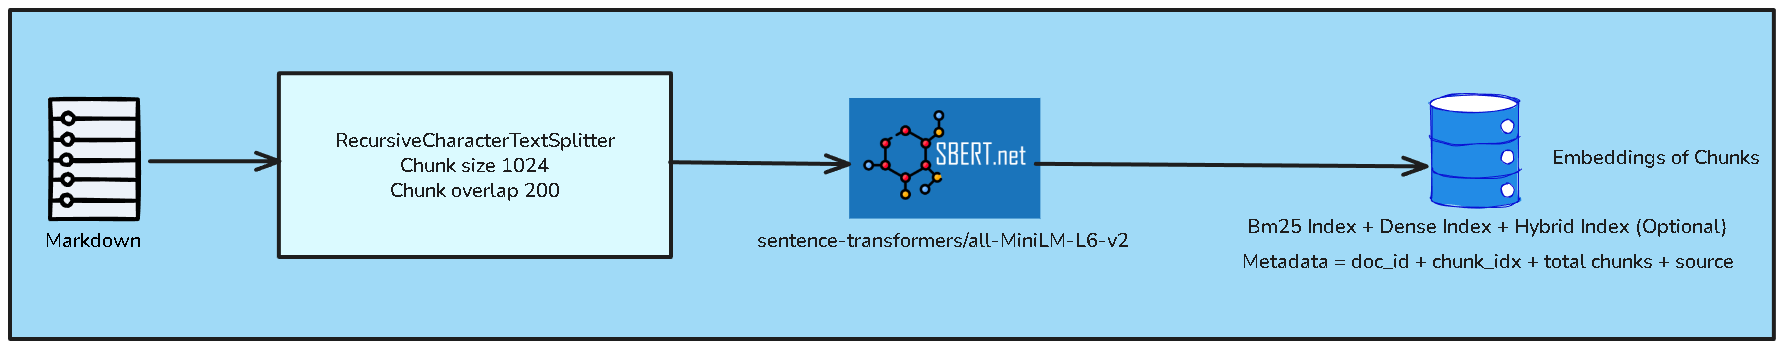
\includegraphics[width=1\textwidth]{img/pdz/20-textchunk.png}
    \caption[Textual Chunking and Embedding]{Textual Chunking and Embedding.}
    \label{fig:textchunk}
\end{figure}

% \textbf{Chunking Logic}

% The system employs the \texttt{RecursiveCharacterTextSplitter} with the following specific configuration:
% \begin{itemize}
%     \item \textbf{Chunk Size}: 1024 characters.
%     \item \textbf{Chunk Overlap}: 200 characters.
% \end{itemize}


Textual data is segmented into chunks to fit within the context window of the embedding models. 
The system employs the \texttt{RecursiveCharacterTextSplitter} with the configuration using a chunk size of 1024 characters with an overlap of 200 characters. 
This overlap ensures semantic continuity across chunk boundaries, preventing context loss for sentences that straddle the split point. 
% The retrieval mechanism is \textit{Hybrid}, combining two distinct algorithms:
% \begin{enumerate}
%     \item \textbf{Sparse Retrieval (BM25)}: Utilizes keyword matching to capture exact terms and domain-specific jargon.
%     \item \textbf{Dense Retrieval}: Utilizes vector embeddings (stored in FAISS indices) to capture semantic meaning and context. The default embedding model is \texttt{all-MiniLM-L6-v2}.
% \end{enumerate}
% Scores from both retrievers are combined using Min-Max normalization and a weighted sum (default $\alpha=0.5$).


\textbf{Text Vectorization (SBERT)}

Processed chunks are mapped to a high-dimensional vector space using the \textbf{Sentence-BERT (SBERT)} framework.
\begin{itemize}
    \item \textbf{Model}: \texttt{sentence-transformers/all-MiniLM-L6-v2}.
    \item \textbf{Output}: A 384-dimensional dense vector representing the semantic meaning of the text chunk.
    \item \textbf{Index Structure}: The embedding is stored alongside a composite metadata object containing:
    \begin{verbatim}
    {
      "doc_id": "unique_document_identifier",
      "chunk_idx": "integer_sequence_number",
      "total_chunks": "total_count_for_document",
      "source": "original_filename"
    }
    \end{verbatim}
\end{itemize}

\textbf{Visual Embedding (ColQwen)}

For documents rich in diagrams, charts, and complex layouts, the pipeline utilizes JPG images derived from the canonical PDF files.
% The system implements a "1 Page = 1 Image" conversion strategy. Each PDF page is rendered as a high-resolution JPEG image.
These intermediate image files are stored temporarily to facilitate the vision-based embedding process used by ColQwen, ensuring the model ``sees'' the document exactly as a human would.


The visual pathway processes the page images generated to enable multimodal retrieval.

\begin{figure}[H]
    \centering
    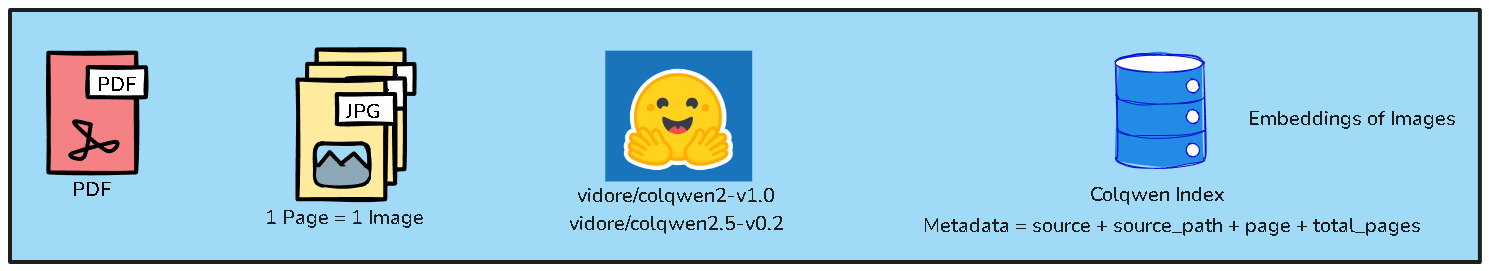
\includegraphics[width=1\textwidth]{img/pdz/21-visualemb.png}
    \caption[Visual Embedding (ColQwen)]{Visual Embedding (ColQwen).}
    \label{fig:visualemb}
\end{figure}

\textbf{Vision-Language Model}

The system integrates the \textbf{ColQwen} architecture (specifically \texttt{vidore/colqwen2-v1.0} or \texttt{v2.5}). Unlike standard OCR which strips layout, ColQwen encodes the visual semantics of the entire page.

\textbf{Visual Indexing}

\begin{itemize}
    \item \textbf{Embedding Process}: Each rasterized page image is passed through the ColQwen vision encoder to produce visual tokens.
    \item \textbf{Storage}: These embeddings are stored in a specialized ColQwen Index.
    \item \textbf{Metadata Schema}: Visual embeddings are tagged with precise location data:
    \begin{verbatim}
    {
      "source": "original_filename",
      "source_path": "file_system_path_to_pdf",
      "page": "page_number",
      "total_pages": "document_length"
    }
    \end{verbatim}
\end{itemize}

\textbf{Hybrid Retrieval Integration}

The retrieval unifies these two streams. 
The Text and Visual indices can be queried simultaneously to return both relevant text snippets and their corresponding visual page contexts.

The index supports \textbf{Hybrid}, allowing for keyword precision and semantic recall, combining two distinct algorithms:

\begin{enumerate}
    \item \textbf{Sparse Retrieval (BM25)}: Utilizes keyword matching to capture exact terms and domain-specific jargon.
    \item \textbf{Dense Retrieval}: Utilizes vector embeddings (stored in FAISS indices) to capture semantic meaning and context. The default embedding model is \texttt{all-MiniLM-L6-v2}.
\end{enumerate}

Scores from both retrievers are combined using Min-Max normalization and a weighted sum.



\section{Database Schema and Storage}
The system implementation requires a robust schema design to manage user interactions, documents, and vector representations. We utilize a dual-database approach, leveraging \textbf{Amazon DynamoDB} for persistent metadata and conversational state, and \textbf{Qdrant} for high-performance vector retrieval.

\subsection{Schema Property Definitions}
Before detailing the specific collection structures, we define the properties utilized within our schema tables to ensure technical clarity.

\begin{table}[H]
    \centering
    \begin{tabular}{llp{8cm}}
        \toprule
        \textbf{Property} & \textbf{Description} & \textbf{Note} \\
        \midrule
        Field & Name of the attribute in the database & Mandatory. \\
        Type & The technical data format & String, Boolean, Enum, or Vector. \\
        Description & Purpose of the field within the system & Context for the specific attribute. \\
        Note & Structural role or indexing constraint & e.g., Primary Key, Partition Key, Sort Key. \\
        \midrule
        Dim & The length of the embedding vector & Mandatory for dense vector fields. \\
        Distance & The distance calculation for retrieval & Mandatory for vector indices (e.g., Cosine). \\
        \bottomrule
    \end{tabular}
    \caption{Schema properties used in implementation documentation}
    \label{tab:schema_props}
\end{table}

\subsection{Vector Storage (Qdrant)}
To support our Hybrid + Multimodal retrieval strategy, we segregate embeddings into dedicated Qdrant collections. Each collection is distinctly configured with dimensions and distance metrics tailored to the deployed embedding model architecture.

\textbf{Collection: \texttt{edu\_text\_chunks}}
Stores granular textual chunks extracted from structured Markdown documents. It utilizes a hybrid search approach, combining sparse keyword indexing with the following dense vector configuration.
\begin{table}[H]
    \centering
    \begin{tabular}{lp{1cm}p{1.8cm}p{5.5cm}}
        \toprule
        \textbf{Vector Name} & \textbf{Dim} & \textbf{Distance} & \textbf{Description} \\
        \midrule
        text & 384 & Cosine & Main text embeddings representing chunk semantics (e.g., via \texttt{all-MiniLM-L6-v2}). \\
        \bottomrule
    \end{tabular}
    \caption{Text Vector Collection Properties}
    \label{tab:qdrant_text}
\end{table}

Each indexed text chunk retains critical metadata necessary for strict multi-tenant filtering and file attribution during generative retrieval:
\begin{table}[H]
    \centering
    \begin{tabular}{llp{8cm}}
        \toprule
        \textbf{Field} & \textbf{Type} & \textbf{Note / Description} \\
        \midrule
        point\_id & UUID & Primary Key. Unique identifier mapped to the vector. \\
        \midrule
        chunk\_id & String & Unique string identifier for the block. \\
        user\_id & String & Tenancy boundary identifier. \\
        source & String & Original filename. \\
        text\_preview & String & Truncated preview of the chunk. \\
        storage\_uri & String & Cloud location of the chunk artifact. \\
        storage\_backend & String & Storage system (e.g., s3). \\
        \bottomrule
    \end{tabular}
    \caption{Text Collection Schema Structure}
    \label{tab:qdrant_text_schema}
\end{table}

\textbf{Collection: \texttt{edu\_image\_pages}}
Dedicated to storing high-order visual layouts. It leverages a unique multi-vector representation generated directly from the ColQwen vision-language model, enabling direct visual similarity searches against original PDF structures.
\begin{table}[H]
    \centering
    \begin{tabular}{lp{1cm}p{1.8cm}p{5.5cm}}
        \toprule
        \textbf{Vector Name} & \textbf{Dim} & \textbf{Distance} & \textbf{Description} \\
        \midrule
        colpali\_multivec & 128 & Dot & Multi-vector representations of visual page elements for ColQwen processing. \\
        \bottomrule
    \end{tabular}
    \caption{Image Vector Collection Properties}
    \label{tab:qdrant_image}
\end{table}

The visual index maintains geometric representations (height/width) alongside S3 references, allowing the orchestration layer to securely retrieve the original page images for multimodal language models:
\begin{table}[H]
    \centering
    \begin{tabular}{llp{8cm}}
        \toprule
        \textbf{Field} & \textbf{Type} & \textbf{Note / Description} \\
        \midrule
        point\_id & UUID & Primary Key. Unique identifier mapped to the vector. \\
        \midrule
        user\_id & String & Tenancy boundary identifier. \\
        source & String & Original document name. \\
        source\_path & String & Absolute physical path of document. \\
        page & Integer & The structural page number. \\
        total\_pages & Integer & The total length of the PDF. \\
        image\_width & Integer & Pixel width of the page boundary. \\
        image\_height & Integer & Pixel height of the page boundary. \\
        storage\_uri & String & Cloud location of the rasterized image. \\
        storage\_backend & String & Storage system (e.g., s3). \\
        \bottomrule
    \end{tabular}
    \caption{Image Collection Schema Structure}
    \label{tab:qdrant_image_schema}
\end{table}

\subsection{Metadata and State Schemas}
Stateful operations are handled across two managed cloud services: DynamoDB for high-throughput chat logging, and Firebase (Firestore) for secure identity and profile management. The following tables outline the primary schemas:

\textbf{Chatbot Sessions Table}
We developed an optimized schema to organize chat histories per user.
\begin{table}[H]
    \centering
    \begin{tabular}{llp{8cm}}
        \toprule
        \textbf{Field} & \textbf{Type} & \textbf{Note / Description} \\
        \midrule
        user\_id & String & Partition Key. Identifies the owner of the chat. \\
        session\_id & String & Sort Key. Unique identifier for the chat session. \\
        \midrule
        title & String & Short text describing the session context. \\
        pinned & Boolean & Indicates whether the user has pinned this chat. \\
        message\_count & Integer & Total number of messages exchanged in this session. \\
        updated\_at & String (ISO) & Timestamp of the last conversational interaction. \\
        \bottomrule
    \end{tabular}
    \caption{Chatbot Sessions Schema}
    \label{tab:chat_sessions}
\end{table}

\textbf{Chatbot Messages Table}
Stores individual conversational turns (prompts and AI responses).
\begin{table}[H]
    \centering
    \begin{tabular}{llp{8cm}}
        \toprule
        \textbf{Field} & \textbf{Type} & \textbf{Note / Description} \\
        \midrule
        session\_id & String & Partition Key. Link to the parent chat session. \\
        message\_id & String & Sort Key. Unique identifier for the message. \\
        \midrule
        role & String & Identifier for sender: \texttt{user}, \texttt{assistant}, or \texttt{system}. \\
        content & String & The Markdown body of the message. \\
        created\_at & String (ISO) & Timestamp identifying the message sequence. \\
        \bottomrule
    \end{tabular}
    \caption{Chatbot Messages Schema}
    \label{tab:chat_messages}
\end{table}

\textbf{User Profile Table (Firestore)}
While conversational data resides in AWS, core authentication layers and user profiles are synchronized securely via Google Firebase. The profile information is critical as it passes user context into the final LLM prompt (e.g., tailoring responses to a university student versus a middle schooler).
\begin{table}[H]
    \centering
    \begin{tabular}{llp{8cm}}
        \toprule
        \textbf{Field} & \textbf{Type} & \textbf{Note / Description} \\
        \midrule
        uid & String & Primary Key. Unique identifier generated and linked to Firebase Auth. \\
        \midrule
        email & String & User's registered email address. \\
        displayName & String & The user's visible display name. \\
        role & Enum & Role definition: \texttt{student}, \texttt{admin}, or \texttt{instructor}. \\
        persona & String & Selected AI persona trait (e.g., Socratic, Direct) to guide the LLM's conversational tone. \\
        educationDescription & String & Academic background provided by the user to adapt explanation complexity. \\
        \bottomrule
    \end{tabular}
    \caption{User Profile Schema}
    \label{tab:user_profiles}
\end{table}


\section{Core API Services}
The core API, built with FastAPI, serves as the communication backend between the frontend UI, the RAG orchestration logic, and the databases.

\subsection{Search and Generation Endpoint [\texttt{POST} \texttt{/api/search/chat}]}

Executes hybrid searches and utilizes local/cloud LLMs to generate contextual answers.
\begin{itemize}
    \item \textbf{query}: Natural language query (e.g., ``Summarize the data fetching section'').
    \item \textbf{top\_k} (optional, default=10): Parameter restricting the document candidate pool size.
    \item \textbf{retriever\_type} (optional, default=``hybrid''): Specifies the search logic (bm25, dense, or hybrid).
    \item \textbf{mode}: Controls the operation (\texttt{retrieval\_only} vs. \texttt{retrieval\_generation}).
\end{itemize}

\textbf{Processing steps:}
\begin{enumerate}
    \item \textbf{Input Validation}: Ensure the query parameters are well-formed and session tokens valid.
    \item \textbf{Hybrid Search}: Execute parallel searches against the Text Collection (combining dense vector cosine similarity with BM25 keyword matching) and the Image Collection (via ColQwen embedding).
    \item \textbf{Prompt Augmentation}: Format the retrieved markdown chunks and visual contexts into an enhanced LLM prompt.
    \item \textbf{Response Generation}: Forward the contextually enriched prompt to the generation provider (e.g., local Ollama or AWS Bedrock) and stream the JSON response back to the client.
    \item \textbf{History Synchronization}: Asynchronously log the interaction into the DynamoDB Chatbot Messages table for persistence.
\end{enumerate}

\subsection{Data Processing Endpoint [\texttt{POST} \texttt{/api/files/process}]}

Initiates the document normalization and structural extraction pipeline.
\begin{itemize}
    \item \textbf{selected\_paths}: Target input files.
    \item \textbf{mode}: ``standard'' (full multimodal) or ``fast'' (text-only).
\end{itemize}

\subsection{Indexing Endpoint [\texttt{POST} \texttt{/api/pipeline/index}]}

Vectorizes processed artifacts (Markdown strings and physical PDF pages) and pushes them into Qdrant storage.
\begin{itemize}
    \item \textbf{mode}: Setting to ``fast'' restricts indexing to Text Collection only to reduce computational overhead if visual diagrams are unneeded.
\end{itemize}

\section{System Configurations and Modular Architecture}

To ensure scalability and adaptability, the backend architecture introduces several configuration modalities that dictate how machine learning operations, multi-tenancy, and file storage are managed.

\subsection{Multi-tenant Architecture and Asset Management}
The system is designed from the ground up to support isolation across multiple concurrent users.
\begin{itemize}
    \item \textbf{Tenant Isolation}: HTTP requests utilize an \texttt{X-User-Id} header to logically isolate data. Qdrant vector collections remain shared but are partitioned using payload filtering by \texttt{user\_id}.
    \item \textbf{Storage Backend (Local vs. S3)}: The system supports two primary storage modes dictated by environmental variables (\texttt{FILE\_STORAGE\_BACKEND}). Small-scale deployments can utilize local filesystem storage (\texttt{backend/input} and \texttt{backend/output}), while production environments seamlessly switch to \textbf{Amazon S3}. When operating in S3 mode, files are logically isolated using key prefixes (e.g., \texttt{users/<user\_id>/...}).
\end{itemize}

\subsection{Inference and Compute Scalability}
The system architecture cleanly decouples the application layer from the heavy inference processing logic.
\begin{itemize}
    \item \textbf{Local Inference}: By default, models such as ColQwen and embedding transformers are loaded locally via GPU/CPU (\texttt{colpali-engine}).
    \item \textbf{AWS SageMaker Integration}: For production-grade scalability, the backend can delegate inference tasks to AWS SageMaker endpoints (\texttt{USE\_AWS\_SAGEMAKER\_INFERENCE=true}). This strategy mitigates API host bottlenecking during intensive tasks like multimodal embedding generation.
\end{itemize}

\subsection{Chat Runtime Environments}
Conversational capabilities are adaptable to different operational frameworks based on the \texttt{CHAT\_AGENT\_RUNTIME} flag:
\begin{itemize}
    \item \textbf{Local Runtime}: The default mode utilizes local logic to handle conversational intelligence.
    \item \textbf{AgentCore Runtime}: Administrators can configure the backend to interact with a deployed AWS Bedrock AgentCore environment. This integrates seamlessly with the DynamoDB session tracking schemas.
\end{itemize}

\subsection{Educational Insights API}
Beyond core Retrieval-Augmented Generation, the system leverages the pipeline's high-fidelity Markdown structural outputs to offer specialized analytical endpoints (under \texttt{/api/insights/*}):
\begin{itemize}
    \item \textbf{Summary Generation [\texttt{POST} \texttt{/api/insights/summary}]}: Generates targeted abstracts with customizable depth, length, and organizational tone based on extracted documents.
    \item \textbf{Multiple Choice Questions [\texttt{POST} \texttt{/api/insights/mcq}]}: Synthesizes quizzes dynamically (including correct answers and rationales) geared toward testing specific proficiency levels.
    \item \textbf{Learning Roadmap [\texttt{POST} \texttt{/api/insights/learning-roadmap}]}: Formulates personalized, step-by-step educational guides tailored to the user's specific goals and professional profile.
\end{itemize}

\newpage